\subsection{Testbild ohne Makroring}
Für diesen Versuch sollen zwei Fotos von einer FH-Karte gemacht werden, zunächst ohne Makroring danach eine Aufnahme mit grossem Makroring, beide Aufnahmen mit einer Brennweite von 108mm.

Leider hat sich herausgestellt das die Aufnahme ohne Makroring nicht richtig abgespeichert wurde, weshalb nur die kürzeste fokussierbare Distanz von Linse zu Objekt vorhanden ist, welche 11.5cm beträgt.

\subsection{Testbild mit Makroring}
Nach dem einsetzen des Makroringes konnte dieselbe Messung nochmal gemacht werden, diesmal beträgt die gemessene Distanz von Linse zu Karte 2cm (siehe Grafik \ref{fig::imMakroring})

\begin{figure}[ht]
	\centering
	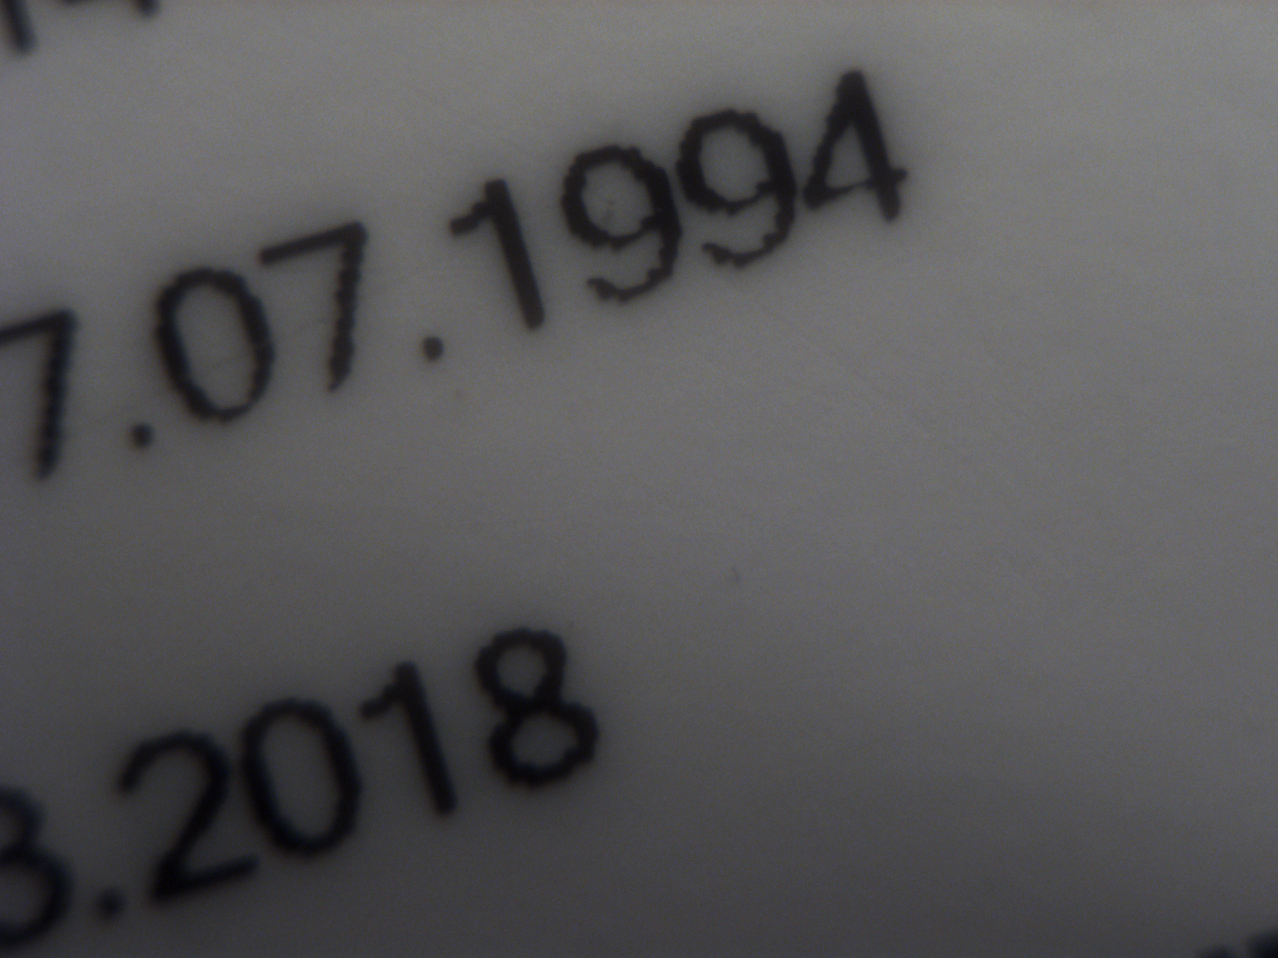
\includegraphics[width=0.8\textwidth]{imMakroring.png}
	\caption{Aufnahme mit eingesetztem Makroring}
	\label{fig::imMakroring}
\end{figure}

\subsection{Fokussieren im Unendlichen}
Als letztes wurde noch untersucht in welchem Bereich das Objekt mit Makroring fokussiert werden kann. Theoretisch sollten zwei Bereiche vorhanden sein in welchem die FH-Karte scharf zu sehen ist, es wurde aber nur der Bereich um 2cm gefunden. Es wurde die Schlussfolgerung gezogen, dass mit dem Makroring Objekte auf kürzere Distanzen scharfgestellt werden können, jedoch die maximale Distanz bei welcher ein Objekt gut zu sehen ist verringert wird